% Szglab4
% ===========================================================================
%
\chapter{Követelmény, projekt, funkcionalitás}

\thispagestyle{fancy}

\section{Követelmény definíció}
\label{sec:reqdef}

\subsection{A program célja, alapvető feladata}

Az általunk kifejlesztett program célja egy előre megadott digitális áramkör szimulációja és annak megjelenítése, grafikus mindenki számára könnyen kezelhető, átlátható formában. Az alkalmazás az áramköri elemekből felépített digitális hálózat működését szemlélteti úgy, hogy felhasználói interakciók során a rendszer bemenetei átkonfigurálhatóak.

\subsection{A fejlesztőkörnyezet}
\label{sec:devenvironment}

A fejlesztéshez NetBeans 6.9.1 szoftvert választottuk. Az UML diagramok elkészítéséhez a Visual Paradigm for UML nevű alkalmazást használjuk, mely képes az osztály-diagramból Java forráskódot generálni és vica versa. Fejlesztés során szem előtt tartjuk, hogy a program kompatibilis legyen az Oracle által gondozott Java 1.6-os verziójával. Természetesen a cél az, hogy a digitális áramkört modellező program a Hallgatói Számítógép Központban rendszeresített JDK és JRE alatt fordítható és futtatható legyen. A dokumentumokat \LaTeX{}-hel készítjük el a Texmaker nevű alkalmazás segítségével, melyet PDF-be fordítunk le. A unit-tesztekre a JUnit csomagot fogjuk használni.

Mivel a fentebb felsoroltak közül mindegyik alkalmazás fut mind Windows, mind Linux operációs rendszeren, így az egész fejlesztés mindkét platformon megvalósítható.

\subsection{A futtatáshoz szükséges környezet}

Java Runtime Environment 1.6-os verziója, illetve az a számítógép, mely ezt futtatni képes. A modellező alkalmazás használatához billentyűzet, grafikus képernyő és egér szükséges.

\subsection{A felhasználói felület}

A program végső változata grafikus felhasználói felülettel rendelkezik. A programot a felhasználó az egér és a billentyűzet segítségével vezérelheti.

\subsection{Minőségi tényezők}

\textbf{Teljesítmény}: A cél az, hogy a digitális rendszermodellező szoftver használható legyen a fentebb meghatározott minimális rendszeren. A grafikus felületnél törekedni fogunk a folyamatos szimuláció megjelenítése.\\
\textbf{Újrafelhasználhatóság}: A cél az, hogy a grafikus felhasználói felületet a program többi részétől teljesen különválasszuk, így lehetővé téve azt, hogy később a grafikus felület egyszerűen és gyorsan változtatható legyen.\\
\textbf{Rugalmasság}: A rugalmasságot a fejlesztőkörnyezet biztosítja, a modellező szoftvernek ugyanis minden olyan környezetben futtathatónak kell lennie, melyben létezik megfelelő Java futtatókörnyezet.\\
\textbf{Felhasználhatóság}: A használat különösebb tanítást nem igényel, alapfokú számítástechnikai tudással akár a felhasználói kézikönyv elolvasása nélkül is használható.

\subsection{A software minősítése}

A kifejlesztett software akkor megfelelő, ha minél pontosabban megegyezik a fentebb leírtakkal. Ezt ellenőrizni lehet a program futtatásával és kipróbálásával, illetve a forráskód és a modell összevetésével, valamint a funkcionális tesztek futtatásával.

\subsection{A kibocsátás}

A program kibocsátása először a forráskóddal együtt a konzulens felé fog történni.

\section{Projekt terv}
\label{sec:projectplan}

\subsection{A fejlesztői csapat}

\begin{center}
\begin{tabular}{l | l}
	\textbf{Csapattag neve} & \textbf{feladatköre} \\
	\hline
	Kriván Bálint & csapatvezető, kód, dokumentáció, szervezés \\ 
	Jákli Gábor & kód, dokumentáció, ticket-koordinátor \\ 
	Dévényi Attila & kód, dokumentáció, GUI-felelős \\ 
	Apagyi Gábor & kód, dokumentáció \\ 
	Péter Tamás Pál & kód, dokumentáció 
\end{tabular}
\end{center}

\subsection{Életciklus modell}

A feladat először a program megtervezése, mely a dinamikus és objektum modelleket foglalja magába. Ha ez készen van, elkezdhető a skeleton implementálása. Ez a lépés már teljesen meghatározott, nem merülhet fel semmilyen komplikáció, ha a modellek megfelelőek voltak.
A következő feladat a prototípus elkészítése. A programnak ebben az állapotban könnyen tesztelhetőnek kell lennie, hogy a programozási és funkcionalitási logikai hibák könnyen felismerhetők legyenek. Ha már a prototípus is megfelelő, akkor kezdődhet a grafikus felület megvalósítása. Itt is fontosa tesztelés és a kiértékelés, mert a jó megjelenés sokat számít a modellező használhatóságában. Ha ennek kifejlesztése is sikeres, készen van a program első teljes változata. A kötelező feladat csak eddig tart. Ezt a változatot kell leadni a dokumentációval és a forráskóddal együtt.

\subsection{Szervezési struktúra}
\label{sec:orgstructure}

A csapat öt emberből áll. A feladat szempontjából a tudásunk nem azonos, mindenki más-más területet érez a magáénak, illetve a feladat eltérő részeinek megoldásához van nagyobb kedvünk. Azt a felépítést választottuk, hogy mindenki az érdeklődésének és tudásának legmegfelelőbb részt kapja az egész feladatból. A feladatok szétosztását találkozókon, illetve az alább meghatározott kommunikációs csatornákon egyeztetjük, ahol az egyéni kívánságok mellett ügyelünk arra, hogy minden feladat kiosztásra kerüljön, valamint a csapattagok az egész feladat megoldásából nagyjából egyenlő mértékben vegyék ki a részüket. A találkozók keretében, mivel a szétosztott feladatok nagy mértékben függnek egymástól, javaslatokat teszünk egymásnak a feladat megoldásának körülményeit és a határidőt illetően.\\

A forráskódot és minden a fejlesztés során elkészülő dokumentációt, illetve a projekthez tartozó egyéb fájlokat megegyezés alapján egy Git központi tárolóban tároljuk, melyhez a Codaset (\url{http://codaset.com}) nevű ingyenes szolgáltatását használjuk és erről mindenki egy saját klónt készít.\\

A kiosztott feladatokat a tulajdonosuk elvégzi a megbeszélt határidőig, de ha ez megváltozott funkcionalitást takar, akkor az adott csapattag köteles a megfelelő teszteseteket megírni, és azok sikeres lefutásáról meggyőződni. Abban az esetben, ha az alkalmazás nem fordul le, vagy valamelyik teszteset nem fut le sikeresen, az adott commit visszaállításra kerülhet annak kijavításáig, melyet a ticket-rendszerben jelezzük a másik felé.\\
\\
Hogy a fejlesztés minél hatékonyabb és zökkenőmentesebb legyen, a következő eszközöket, technológiákat alkalmazzuk:
\begin{description}
\item[E-mail] Az egymás számára fontos anyagokat, melyeket a találkozókon előzetesen megbeszéltünk, levélben küldjük el.
\item[Msn] Felvettük egymást a Microsoft Messenger-be, hogy szükség esetén egymástól is segítséget tudjunk kérni kisebb technikai problémák megoldásában. Természetesen ezek a feladat lényegét, a projektről hozott döntéseket nem érinthetik, de kivételes helyzetben akár az Interneten is tarthatunk találkozót.
\begin{figure}[h]
\begin{center}
\includegraphics{chapters/chapter02/msn.png}
\caption{MSN csoport a csapatnak}
\label{fig:msn}
\vspace{-20pt}
\end{center}
\end{figure}
\item[Git tároló] A feladatok megoldása közben keletkezett anyagokat egy -- kizárólag a csapat tagjai által hozzáférhető -- helyen tároljuk (lásd fentebb). Így mindig elérhető a fejlesztések legfrissebb változata.
\begin{figure}[h]
\begin{center}
\includegraphics[width=10cm]{chapters/chapter02/git.png}
\caption{Git történet}
\label{fig:git}
\vspace{-20pt}
\end{center}
\end{figure}
\item[Ticket-rendszer] A fejlesztés során felmerülő problémákat, kérdéseket ticket formájában megírjuk egymásnak, amit később a kijelölt felelős személy megold, ha szükséges, akkor együtt konzultálunk a megoldás módjáról, menetéről.
\begin{figure}[h]
\begin{center}
\includegraphics[width=16.7cm]{chapters/chapter02/ticket.png}
\caption{Ticketek}
\label{fig:ticket}
\vspace{-20pt}
\end{center}
\end{figure}
\end{description}

\subsection{Fejlesztési ütemterv}

A program fejlesztésének három fő lépcsőfoka van. Ezek a következők:\\
\textbf{Skeleton}: A cél az, hogy mind a dinamikus, mind az objektum modell jól legyen kitalálva. Ha ezek elkészültek, akkor a fejlesztés szempontjából sikeresen leraktuk az alapokat.\\
\textbf{Prototípus}: Ez már szinte a teljes változat, csak a grafikus felület elemei hiányoznak. Ez a változat tökéletesen megfelelő arra, hogy az objektumok, rutinok, függvények szemantikai helyességét vizsgáljuk.\\
\textbf{Grafikus változat}: A program teljes változata. Tulajdonképpen a prototípus a grafikus felülettel kiegészítve, esetleg kismértékben továbbfejlesztve.

\subsection{Határidők}

\begin{tabular}{l | l}
febr. 11. & Csapat regisztráció \\
febr. 21. & Követelmény, projekt, funkcionalitás \\
febr. 28. & Analízis modell kidolgozása 1. \\
márc. 7. & Analízis modell kidolgozása 2. \\
márc. 14. & Szkeleton tervezése \\
márc. 21. & Szkeleton \\
márc. 28. & Prototípus koncepciója \\
ápr.  4. & Részletes tervek \\
ápr. 18. & Prototípus \\
ápr. 26. & Grafikus felület specifikációja \\
máj. 9. & Grafikus változat \\
máj. 13. & Összefoglalás
\end{tabular}

\section{Feladatleírás}
\label{sec:taskdesc}

Az általunk készített alkalmazás segítségével a felhasználó egy előre elkészített áramköri listából kiválasztott digitális áramkör szimulációját végezheti el grafikus megjelenítéssel. A program az alábbi alkatrészeket támogatja áramköri elemként: ÉS kapu, VAGY kapu, Inverter, Kijelző, Jelgenerátor, Kapcsoló, Vcc és Gnd. Ezek mindegyike egy vagy több ki- és/vagy bemenettel rendelkezik.\\

\noindent A komponensek (alkatrészek) részletezése:

\begin{enumerate}
\item \textbf{Általános komponensek}: A bemenet(ek)re érkező logikai érték(ek) alapján a kimenete(ke)n valamilyen logikai érték(ek)et produkálnak.
\begin{itemize}
\setlength{\itemsep}{0cm}%
\setlength{\parskip}{0cm}%
\item Az ÉS kapu kettő vagy több bemenettel és egy kimenettel rendelkezik. A kimeneten a bemenetre kötött jelek logikai ÉS kapcsolata jelenik meg. 
\item A VAGY kapu kettő vagy több bemenettel és egy kimenettel rendelkezik. A kimeneten a bemenetre kötött jelek logikai VAGY kapcsolata jelenik meg.
\item Az Inverter egyetlen kimenetén az egyetlen bemenetére kötött jel logikai negáltja jelenik meg.
\end{itemize}

\item \textbf{Megjelenítők}: Az ide tartozó elemek feladata a logikai értékek vizualizálása
\begin{itemize}
\setlength{\itemsep}{0cm}%
\setlength{\parskip}{0cm}%
\item A Kijelző komponenssel a felhasználó a bemenetre kötött jelet vizuális formában tudja megjeleníteni.
\end{itemize}

\item \textbf{Jelforrások}: A harmadik csoport elemei melyeknek nincs bemenete csak kimenete, ez vagy előre definiált (gnd és vcc) vagy a felhasználó által módosítható (kapcsoló, jelgenerátor), ezáltal változtatva az áramkör működését.
\begin{itemize}
\setlength{\itemsep}{0cm}%
\setlength{\parskip}{0cm}%
\item Jelgenerátor segítségével egy bitsorozatot tárolhatunk el, amelyet a szimuláció során az egyetlen kimenetén ciklikusan kiad.
\item A Kapcsolónak egy kimenete van, melynek értéke a kapcsoló állásától függ. „Be” állásban igaz, „Ki” állásban hamis értékű.
\item Gnd (,,föld'') konstans 0-át (logikai hamis) kiadó jelforrás.
\item Vcc (,,tápfeszültség'') konstans 1-et (logikai igaz) kiadó jelforrás.
\end{itemize}
\end{enumerate}

Az összes alkatrészre igaz, hogy nem lehet olyan bemenetük, amelyek szabadok, vagyis sehova sincsenek bekötve, ellenkező esetben a szimulációt nem lehet elindítani és a program figyelmezteti erre a felhasználót (ennek elkerülésére, a programmal szállított szimulálható áramkörök egyik komponensének sincs szabad bemenete).

A felhasználó a fentebb említett alkatrészekből összeállított digitális áramkör szimulációját végezheti. Az alkatrészek és azok egymáshoz kötéseik (összeköttetések) grafikus formában kerül megjelenítésre.

A szimuláció során bármelyik komponens pillanatnyi értékeit a felhasználó lekérdezheti az alkatrészre való kattintással, ezzel egyidejűleg a szimulációt szünetelteti. Az áramkör vizsgálata közben a Kapcsolók értékeit szabadon változtathatja, melyek hatása valós időben megjelenik. Szimuláció elkezdésekor az összes áramköri elem kimenete hamis értéket vesz fel. Ha a vizsgálandó áramkör bizonyos idő alatt nem áll be stacionárius állapotba változatlan bemenetek mellett, akkor ez jelzésre kerül a felhasználó számára és a szimuláció automatikusan leáll. A szimuláció bármikor megszakítható majd újraindítható, illetve átválthat egy másik digitális áramkör vizsgálatára (az előre elkészített digitális áramkörök közül választva), amennyiben a jelenlegi áramkört nem kívánja tovább használni.

A szimuláció sebessége a felhasználó által konfigurálható, ezáltal a Jelgenerátor kimenetein kiadott jelek váltakozásának sebessége változtatható.

A Kapcsolók, illetve a Jelgenerátorok gyors és egyszerű alap állapotba helyezése érdekében lehet törölni minden addig elvégzett beállítást egyetlen paranccsal, majd elölről kezdeni az egyes elemek konfigurálását. Lehetőség lesz továbbá a szerkeszthető jelforrások beállításainak elmentésére illetve későbbi visszatöltésére is. A konfiguráció sikeres betöltődéséhez teljesülnie kell annak a feltételnek, hogy abban az összes meghatározott elem szerepeljen az áramkörben, amire használni szeretnénk a beállításokat. Amennyiben ez nem áll fent, akkor a nem specifikált jelforrások alapállapotban lesznek. Előfordulhat még, hogy a konfigurációban olyan elemek szerepelnek, amelyek az áramkörünkben nem, ekkor hibaüzenet jelenik meg és a betöltés megszakad.

\section{Szótár}
\label{sec:dictionary}

\begin{longtable}{r p{10.95cm}}
\textbf{Előre elkészített lista} & Áramköröket tartalmazó előre elkészített gyűjtemény. \\
\textbf{Áramkör} & A komponensek egymáshoz kötéséből létrejövő rendszer. \\
\textbf{Komponens} & Az áramkör alapegysége, mely 3 fajtájú lehet: \emph{általános komponens}, \emph{megjelenítő} és \emph{jelforrás}. \\
\textbf{Alkatrész} & komponens szinonimája\\
\textbf{Általános komponens} & Olyan komponens, mely a bemenet(ek)re érkező logikai érték(ek) alapján a kimenete(ke)n valamilyen logikai érték(ek)et produkál.\\
\textbf{Bemenet} & A komponensek olyan része, melyen keresztül logikai jeleket tudnak fogadni egy másik komponenstől és ezt valamilyen formában felhasználni. \\
\textbf{Logikai jel} & Az áramkörben levő komponensek által továbbított információ a többi komponens számára, mely az igaz illetve a hamis értéket veheti fel.\\
\textbf{Igaz érték} & A kétféle logikai jel egyike. (van amikor az '1'-es szimbólum jelöli)\\
\textbf{Hamis érték} & A kétféle logikai jel egyike. (van amikor a '0'-ás szimbólum jelöli)\\
\textbf{Logikai negált} & Az igaz érték logikai negáltja hamis, hamis értéké pedig igaz.\\
\textbf{Kimenet} & A komponens olyan része, melyen keresztül logikai jeleket tud továbbítani más komponenseknek.\\
\textbf{Jel továbbítás} & A logikai jel egyik komponenstől másik komponensig való áramlása.\\
\textbf{Megjelenítő} & Olyan komponens, mely a bemenet(ek)re érkező logikai jele(ke)t a felhasználó számára érzékelhető módon szemlélteti.\\
\textbf{Jelforrás} & Olyan komponens, mely bemenet nélkül továbbítja az áramkörben specifikált vagy a felhasználó által megadott jele(ek)t a kimenetén további komponens(ek) számára. \\
\textbf{Gnd} & Olyan komponens, mely konstans 0-át ad ki a kimenetén. \\
\textbf{Vcc} & Olyan komponens, mely konstans 1-et ad ki a kimenetén. \\
\textbf{Komponensek egymáshoz kötése} & Egy olyan folyamat, amely során 2 komponenst oly módon kapcso\-lunk össze, hogy az egyik komponens bemenetére a másik komponens kimenetének logikai jelét kapja meg.\\
\textbf{Grafikus megjelenítés} & Az áramkör felhasználó számára felfogható, érzékelhető megjelenítése.\\
\textbf{ÉS kapu} & \emph{Általános komponens}, melynek a bemenetére érkező logikai jelek közt található hamis érték, akkor kimenetén hamis értéket, ellenkező esetben (vagyis minden bemenete logikai igaz) igaz értéket továbbít. \\
\textbf{VAGY kapu} & \emph{Általános komponens}, melynek a bemenetére érkező logikai jelek közt található igaz érték, akkor kimenetén igaz értéket, ellenkező esetben (vagyis minden bemenete logikai hamis) haimis értéket továbbít. \\
\textbf{Inverter} & \emph{Általános komponens}, mely a bemenetére érkező logikai jel negáltját továbbítja a kimenetén. \\
\textbf{Kijelző} & Egy darab logikai jelet váró \emph{megjelenítő}, mely logikai igaz bemenet esetén világít (piros, kék vagy sárga színnel, melyet az áramkör leírója határoz meg), hamis esetén nem. \\
\textbf{Áramkör leíró} & Egy olyan szöveg, mely a program által elvárt módon leírja a teljes áramkört a komponensek és azok összeköttetéseinek definiálásával. \\
\textbf{Jelgenerátor} & Olyan \emph{jelforrás}, mely előre megadott bitsorozatot ad ki ciklikusan a kimenetén.\\
\textbf{Bitsorozat} & Logikai jelekből létrejövő olyan sorozat, melynél az igaz értéket ’1’ szimbólum reprezentál, míg a hamis értéket ’0’.\\
\textbf{Kapcsoló} & Olyan \emph{jelforrás}, mely felhasználói interakció hatására kimenetén igaz, vagy hamis értéket továbbít. \\
\textbf{Felhasználói interakció} & Olyan esemény, melyet a felhasználó saját maga vált ki valamely tevékenysége során, ezzel potenciálisan befolyásolva az áramkör működését. \\
\textbf{Szimuláció} & Az a folyamat, mely során minden alkatrész kimenetének logikai jel értékét kiszámoljuk a bemenetére érkező logikai jelekből, vagy ha \emph{megjelenítő}ről van szó, akkor a felhasználó számára a megjelenítő által meghatározott módon szemléltetjük a bemenetére érkező jeleket. Eközben a felhasználó által megadott időközönként (szimuláció sebessége) léptetjük a jelgenerátort. A szimuláció a felhasználó által indítható és megállítható.\\
\textbf{Jelgenerátor léptetése} & A jelgenerátorban tárolt bitsorozat következő elemére lépünk és azt adjuk ki a kimenetén, ha a végére értünk, akkor előlről indul.\\
\textbf{Szimuláció sebessége} & A jelgenerátor egyes állapotai közötti váltás sebessége. \\
\textbf{Valós időben} & A felhasználó számára lényegében érzékelhetetlen idő alatt.\\
\textbf{Stacionárius} & A rendszer egy stabil állapota, melyben olyan értékek jelennek meg a komponensek kimenetein, amelyek hatására (visszacsatolás esetén sem) változiknak a rendszer komponenseinek kimeneti értékei (Jelgenerátor esetén nincs stacionárius állapot)\\
\textbf{Szimuláció megszakítása/leállítása} & A rendszer komponenseinek állapota nem változik, azok a megszakítás pillanatában felvett értékeket mutatják a következő indításig.\\
\textbf{Állapot} & Az áramkör komponenseinek aktuális tulajdonságainak (kimeneti/bemeneti értékek) összessége \\
\textbf{Alap állapot} & Az a kiindulási állapot, mely az áramkör betöltése után keletkezik. Ilyenkor az \emph{általános komponens}ek kimenetén a hamis érték van.\\
\textbf{Jelforrások konfigurációja} & A szerkeszthető jelforrások beállításainak (kapcsolók állapota, jelgenerátorok bitsorozata stb.) egy állapota.
\end{longtable}

\section{Essential use-case-ek}

\subsection{Use-case diagram}
\label{sec:usecasediagram}

\begin{figure}[H]
\begin{center}
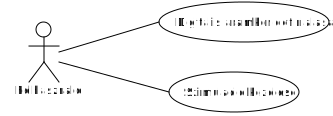
\includegraphics{chapters/chapter02/usecase.pdf}
\caption{Essential use-case diagram}
\label{fig:useCase1}
\end{center}
\end{figure}

\subsection{Use-case leírások}
\label{sec:usecasedesc}

\usecase{Szimuláció leállítás}
{A futó szimuláció leállítása}
{Felhasználó}
{Az éppen futó szimulációt a felhasználó a "Stop" gombbal leállítja.}

\usecase{Szimuláció indítás}
{A áramkör szimulációjának elindítása}
{Felhasználó}
{A felhasználó, az általa korábban kiválasztott áramkör szimulációját a "Start" gombbal elindítja}

\usecase{Áramkör választás}
{Szimulálni kívánt áramkör kiválasztása}
{Felhasználó}
{\vspace{-20pt}\begin{enumerate}
\setlength{\itemsep}{0cm}%
\setlength{\parskip}{0cm}%
\item A felhasználó a Megnyitás menüpontra kapcsol.
\item Kiválaszt egy áramkört a felkínált listából.
\item Az áramkör betöltődik a rendszerbe.
\end{enumerate}\vspace{-20pt}}

\usecase{Jelforrások betöltése}
{Az áramkör jelforrásainak betöltése}
{Felhasználó}
{\vspace{-20pt}\begin{enumerate}
\setlength{\itemsep}{0cm}%
\setlength{\parskip}{0cm}%
\item A felhasználó a "Jelforrások betöltése" menüpontra kapcsol.
\item Megadja, hogy melyik fájlt olvassa be a rendszer.
\item Ha a fájl megfelelő, akkor a betöltés megtörténik, egyéb esetben a felhasználót figyelmeztetjük.
\end{enumerate}\vspace{-20pt}}

\usecase{Jelforrások mentése}
{Az áramkör jelforrásainak mentése}
{Felhasználó}
{\vspace{-20pt}\begin{enumerate}
\setlength{\itemsep}{0cm}%
\setlength{\parskip}{0cm}%
\item A felhasználó a "Jelforrások mentése" menüpontra kapcsol.
\item Megadja, hogy melyik fájlba történjen a mentés.
\item A mentés megtörténik, amennyiben ez valami oknál fogva nem sikerült (nincs joga, nincs elég terület stb.), a felhasználót figyelmeztetjük.
\end{enumerate}\vspace{-20pt}}

